\section{Технический проект}
\subsection{Общая характеристика организации решения задачи}

Разрабатываемая система представляет собой настольное приложение, позволяющее пользователю выполнять две ключевые задачи: построение карт нормалей по двумерным изображениям и интерактивную визуализацию полученных данных с имитацией освещения \cite{tidwell2020}.

Архитектура приложения построена по модульному принципу, что обеспечивает независимость компонентов, удобство расширения и тестирования, а также простоту поддержки. Вся логика работы разделена на два ключевых функциональных блока:

\begin{enumerate}
	\item Модуль генерации карт нормалей. Этот компонент отвечает за обработку загруженного 2D-изображения и построение карты нормалей с помощью градиентного анализа. Пользователь может выбрать один из трёх алгоритмов: Sobel, Scharr или Prewitt. Каждый из них позволяет выявлять локальные изменения яркости изображения и формировать на их основе вектор нормали. В дополнение к алгоритму доступны параметры настройки: сила нормалей, глубина, инверсия. Все изменения применяются в реальном времени, что позволяет интерактивно наблюдать результат и адаптировать карту под нужды конкретной текстуры. Полученная карта нормалей автоматически сохраняется в памяти и используется далее при визуализации.
	\item Модуль визуализации предоставляет пользователю два режима анализа результатов: 2D-визуализацию и 3D-визуализацию.
	\begin{enumerate}[label=\theenumi.\arabic*.]
		\item В 2D-режиме используется техника имитации направленного света («фонарика»), управляемого движением курсора мыши. На основе нормалей рассчитывается освещённость каждой точки изображения, учитывая интенсивность и радиус света, а также уровень фоновой засветки. Таким образом создаётся реалистичный эффект освещения, позволяющий оценить, как текстура будет выглядеть в игровых сценах.
		\item В 3D-режиме карта нормалей и текстура проецируются на все шесть граней виртуального куба, который визуализируется с использованием OpenGL посредством GLCubeWidget. Пользователь может вращать куб мышью, изменяя ракурс наблюдения, и наблюдать взаимодействие нормалей с направленным освещением. Параметры света остаются настраиваемыми -- интенсивность, радиус действия и рассеянность. Это расширяет возможности анализа и делает приложение более гибким в применении к задачам геймдизайна и графического моделирования.
	\end{enumerate}
\end{enumerate}

Поддержка как 2D-, так и 3D-визуализации позволяет пользователю выбирать наиболее подходящий способ анализа текстуры в зависимости от задачи: от быстрой проверки нормалей в плоскости -- до полноценного пространственного анализа поведения света. Такое архитектурное разделение обеспечивает гибкость, модульность и расширяемость приложения.

Графический интерфейс реализован с использованием библиотеки PyQt5 и спроектирован с учётом требований к удобству пользователя \cite{prokhorenok2021}. Все элементы интерфейса размещены логично: процесс работы разбит на этапы (загрузка изображения, генерация нормалей, визуализация), элементы управления параметрами имеют понятные подписи и расположение, соответствующее разработанному макету \cite{cooper2020}.
\subsection{Обоснование выбора технологий проектирования}

При разработке программно-информационной системы создания карт нормалей и их визуализации был проведён анализ различных языков программирования и программных библиотек, применимых для решения задач в области компьютерной графики, обработки изображений и создания пользовательского интерфейса. В результате был выбран стек технологий, оптимально сочетающий простоту разработки, функциональные возможности и широкую поддержку со стороны сообщества.
\subsubsection{Язык программирования: Python}

Python был выбран как основной язык разработки благодаря своей читаемости, лаконичному синтаксису и возможности быстрой реализации алгоритмов, что особенно важно при построении интерактивных приложений. Он активно используется в научных и прикладных областях, включая обработку изображений, машинное обучение и визуализацию данных. Кроме того, кроссплатформенность Python позволяет запускать приложение на различных операционных системах, а большое сообщество и развитая экосистема делают процесс разработки и отладки значительно проще \cite{ravichandiran2020}.
\subsubsection{PyQt5}

PyQt5 -- библиотека для создания графического интерфейса. Для реализации графического интерфейса была выбрана библиотека PyQt5 -- привязка Python к мощному C++ фреймворку Qt \cite{talipov2020}. Основные причины выбора:
\begin{enumerate}
	\item Поддержка широкого спектра элементов интерфейса: кнопки, панели, слайдеры, вкладки и другие виджеты.
	\item Гибкая настройка расположения элементов -- реализована возможность построения интерфейсов, соответствующих пользовательским макетам.
	\item Событийно-ориентированная модель -- облегчает обработку пользовательских взаимодействий (например, загрузка изображений, перемещение мыши).
	\item Интеграция с другими библиотеками Python -- PyQt5 хорошо работает в связке с NumPy, OpenCV и другими модулями.
\end{enumerate}
\subsubsection{OpenCV и NumPy}

OpenCV и NumPy -- библиотеки для обработки изображений. Для обработки изображений и реализации операторов градиентного анализа были использованы библиотеки:
\begin{enumerate}
	\item OpenCV -- открытая библиотека для обработки изображений и компьютерного зрения \cite{kaehler2021}. Обеспечивает эффективную реализацию операторов Sobel, Scharr и Prewitt, а также позволяет выполнять фильтрацию, преобразования, нормализацию и другие операции.
	\item NumPy -- библиотека для работы с многомерными массивами и матрицами. Активно используется для хранения изображений в числовом формате, выполнения математических операций над данными пикселей и ускорения вычислений.
\end{enumerate}
\subsubsection{Pillow}

Pillow -- библиотека для загрузки и сохранения изображений. Для работы с форматами изображений (PNG, JPG и др.) используется библиотека Pillow, являющаяся модернизированной и расширенной версией PIL (Python Imaging Library). Она позволяет:
\begin{enumerate}
	\item Загружать изображения из файлов.
	\item Конвертировать изображения между различными цветовыми пространствами.
	\item Сохранять результаты генерации нормалей в различных форматах.
	\item Извлекать метаинформацию об изображениях.
\end{enumerate}

\subsubsection{OpenGL}
OpenGL -- библиотека для трёхмерной графики и визуализации.
С использованием OpenGL реализованы следующие возможности:
\begin{enumerate}
	\item Создание 3D-сцены с кубом, каждая грань которого текстурирована загруженным изображением.
	\item Назначение карты нормалей в качестве источника данных для расчёта взаимодействия поверхности с направленным освещением.
	\item Обработка пользовательского ввода (вращение, масштабирование сцены).
	\item Моделирование поведения направленного источника света и реалистичного освещения с учётом нормалей.
\end{enumerate}
\begin{comment}
Python был выбран в качестве основного языка разработки по следующим причинам:
\begin{enumerate}
	\item Простота синтаксиса и высокая читаемость кода — это позволяет быстро реализовывать алгоритмы, минимизируя вероятность ошибок и снижая порог входа для других разработчиков \cite{ravichandiran2020}.
	\item Большое количество библиотек для работы с изображениями и интерфейсом — Python активно используется в научной и прикладной разработке в области компьютерного зрения.
	\item Кроссплатформенность — Python-приложения можно запускать под различными операционными системами, включая Windows, Linux и macOS.
	\item Активное сообщество и широкая документация — в случае возникновения проблем легко найти решение или получить помощь.
\end{enumerate}
\subsubsection{PyQt5}

PyQt5 — библиотека для создания графического интерфейса. Для реализации графического интерфейса была выбрана библиотека PyQt5 — привязка Python к мощному C++ фреймворку Qt \cite{talipov2020}. Основные причины выбора:
\begin{enumerate}
	\item Поддержка широкого спектра элементов интерфейса: кнопки, панели, слайдеры, вкладки и другие виджеты.
	\item Гибкая настройка расположения элементов — реализована возможность построения интерфейсов, соответствующих пользовательским макетам.
	\item Событийно-ориентированная модель — облегчает обработку пользовательских взаимодействий (например, загрузка изображений, перемещение мыши).
	\item Интеграция с другими библиотеками Python — PyQt5 хорошо работает в связке с NumPy, OpenCV и другими модулями.
\end{enumerate}
\subsubsection{OpenCV и NumPy}

OpenCV и NumPy — библиотеки для обработки изображений. Для обработки изображений и реализации операторов градиентного анализа были использованы библиотеки:
\begin{enumerate}
	\item OpenCV — открытая библиотека для обработки изображений и компьютерного зрения \cite{kaehler2021}. Обеспечивает эффективную реализацию операторов Sobel, Scharr и Prewitt, а также позволяет выполнять фильтрацию, преобразования, нормализацию и другие операции.
	\item NumPy — библиотека для работы с многомерными массивами и матрицами. Активно используется для хранения изображений в числовом формате, выполнения математических операций над данными пикселей и ускорения вычислений.
\end{enumerate}
\subsubsection{Pillow}

Pillow — библиотека для загрузки и сохранения изображений. Для работы с форматами изображений (PNG, JPG и др.) используется библиотека Pillow, являющаяся модернизированной и расширенной версией PIL (Python Imaging Library). Она позволяет:
\begin{enumerate}
	\item Загружать изображения из файлов.
	\item Конвертировать изображения между различными цветовыми пространствами.
	\item Сохранять результаты генерации нормалей в различных форматах.
	\item Извлекать метаинформацию об изображениях.
\end{enumerate}

OpenGL — библиотека для трёхмерной графики и визуализации.
С использованием OpenGL реализованы следующие возможности:
\begin{enumerate}
	\item Создание 3D-сцены с кубом, каждая грань которого текстурирована загруженным изображением.
	\item Назначение карты нормалей в качестве источника данных для расчёта взаимодействия поверхности с направленным освещением.
	\item Обработка пользовательского ввода (вращение, масштабирование сцены).
	\item Моделирование поведения направленного источника света и реалистичного освещения с учётом нормалей.
\end{enumerate}

Для отображения визуального эффекта освещения по нормалям применяется рендеринг на холст с использованием комбинации данных карты нормалей и положения мыши. Алгоритм реализован вручную с использованием NumPy и PyQt5, без сторонних движков визуализации, что обеспечивает наглядность и полный контроль над процессом.
\end{comment}
\subsection{Общая архитектура системы}

Программно-информационная система генерации карт нормалей и их интерактивной визуализации построена по модульному принципу. Это обеспечивает высокую модульность, возможность масштабирования и упрощает сопровождение и тестирование. Приложение реализовано как настольное, с графическим интерфейсом на языке Python. Система поддерживает два режима визуализации: в 2D с имитацией освещения и в 3D с использованием OpenGL.

Диаграмма компонентов представлена на рисунке~\ref{comp2:image}.

\begin{figure}[ht]
	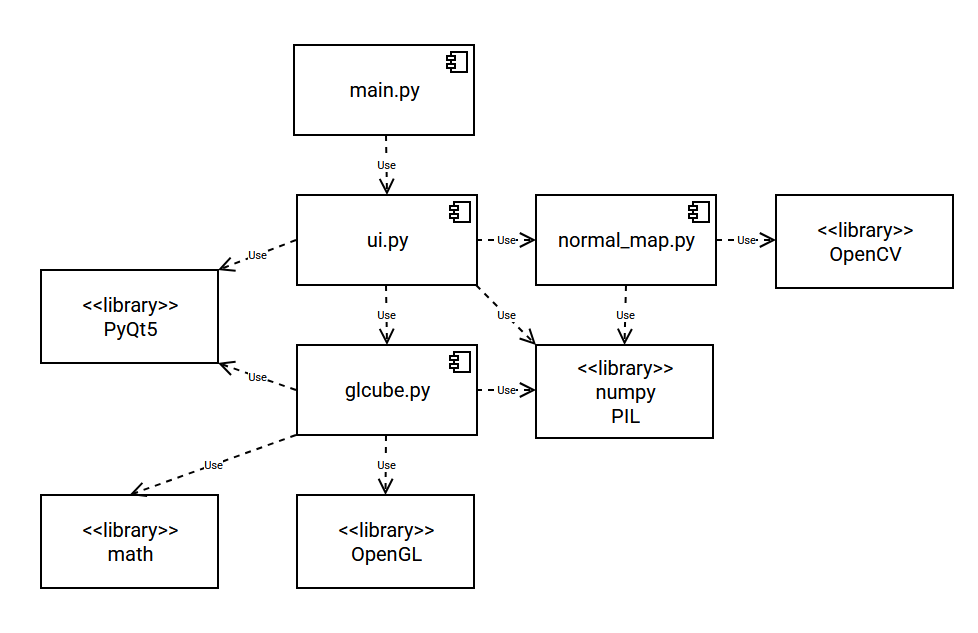
\includegraphics[width=1\linewidth]{comp2}
	\caption{Диаграмма компонентов программной системы}
	\label{comp2:image}
\end{figure}

Основные модули системы:

\begin{enumerate}
	\item Интерфейсный и логический модуль -- файл ui.py.
	\item Модуль генерации карты нормалей -- файл normal\_map.py.
	\item Модуль визуализации в 3D -- файл glcube.py.
	\item Точка входа в приложение -- файл main.py.
\end{enumerate}

\subsubsection{Интерфейсный и логический модуль (ui.py)}

Этот модуль содержит основную логику работы программы и формирует графический интерфейс при помощи библиотеки PyQt5. Все взаимодействия с пользователем происходят именно в этом модуле: действия передаются в модуль генерации нормалей или в OpenGL-виджет. В ui.py реализованы:

\begin{enumerate}
	\item Загрузка изображения (PNG, JPEG, BMP) через диалог выбора файла.
	\item Управление параметрами генерации карты нормалей: выбор оператора (Sobel, Scharr, Prewitt), сила, глубина, инверсия.
	\item Отображение оригинального изображения и сгенерированной карты нормалей.
	\item Визуализация эффекта освещения в 2D режиме -- поведение источника света («фонарика») следует за движением курсора.
	\item Отображение изображения с освещением в реальном времени.
	\item Переключение между 2D и 3D режимами.
	\item Сохранение сгенерированной карты нормалей.
\end{enumerate}

\subsubsection{Модуль генерации нормалей (normal\_map.py)}

Функциональность, связанная с построением карты нормалей на основе изображения, реализована в модуле normal\_map.py. Он предоставляет реализацию нескольких алгоритмов обработки: оператор Собеля, позволяющий вычислять производные первого порядка, оператор Шарра -- более чувствительный к границам, а также оператор Превитта -- простой, но быстрый метод вычисления градиентов. Эти методы позволяют проанализировать локальные изменения яркости изображения и, на их основе, сформировать векторные направления.

Модуль принимает на вход изображение, масштабирует и анализирует его, а затем создаёт нормаль-карту -- изображение, в котором каждый пиксель содержит направление нормали, закодированное в цветовых каналах RGB. Пользователь может регулировать параметры: сила нормалей определяет масштаб по осям X и Y, глубина влияет на составляющую по оси Z, а параметр инверсии меняет направление нормалей на противоположное. Этот модуль полностью автономен и предоставляет интерфейс для подключения к визуализаторам.
\subsubsection{Модуль визуализации в 3D (glcube.py)}

Трёхмерный режим работы реализован в модуле glcube.py, где используется QOpenGLWidget в связке с библиотекой PyOpenGL. Этот компонент отвечает за отрисовку куба, на грани которого накладываются текстура и карта нормалей. Задача -- предоставить пользователю возможность оценить, как освещение взаимодействует с нормалями в пространстве. Модуль осуществляет преобразование изображений в формат, пригодный для загрузки в виде OpenGL-текстур, после чего каждая грань куба получает свой визуальный слой.

Пользователь может вращать куб мышью, изменять масштаб изображения, управлять положением виртуального источника света. Благодаря встроенным функциям расчёта взаимодействия света с нормалями создаётся реалистичная симуляция поведения материала под разными углами обзора и освещённости. Это расширяет возможности анализа и делает приложение полезным в задачах трёхмерного дизайна и текстурирования.

\subsubsection{Точка входа (main.py)}

Файл main.py играет вспомогательную роль. Он содержит лишь минимальный код, необходимый для запуска программы. Основной задачей данного файла является импорт основного класса интерфейса из ui.py, инициализация приложения и передача управления в главный цикл событий. Таким образом, этот модуль является точкой входа в систему и отвечает за запуск всей программной инфраструктуры.
\subsection{Реализация модуля генерации карт нормалей}

Модуль генерации нормалей выполняет задачу преобразования двухмерного изображения в нормал-карту -- изображение с закодированной информацией о направлении нормалей к условной поверхности. Это позволяет воссоздавать визуальное ощущение рельефа без увеличения геометрической сложности сцены \cite{russ2020}.

Алгоритм построения нормалей реализован в несколько этапов, последовательно обрабатывающих входное изображение.

На первом шаге происходит преобразование изображения в полутоновый формат. Перевод в оттенки серого необходим для устранения цветовой информации, которая не влияет на вычисление нормалей, и упрощает последующие операции. Далее изображение представляется в виде числового массива яркостных значений, пригодного для вычислений.

Следующий этап включает расчёт градиентов яркости по горизонтальной и вертикальной осям. Для этого применяется один из стандартных операторов свёртки -- Sobel, Scharr или Prewitt. Выбор осуществляется пользователем через интерфейс приложения. Эти операторы определяют направление и интенсивность изменения яркости, что позволяет судить о локальной «высоте» каждого участка изображения.

Вычисленные значения градиента масштабируются по заданному пользователем параметру силы нормалей. Этот параметр влияет на степень выраженности рельефа: чем выше значение, тем сильнее акцентируются перепады высоты. Компонента нормали вдоль оси Z (глубины) берётся как константа, модифицируемая параметром глубины.

На основе всех трёх компонент (X, Y, Z) формируется вектор нормали. Все векторы проходят процедуру нормализации, приводящую их к единичной длине. Это необходимо для корректной интерпретации направлений в графической визуализации.

Дополнительно реализована опция инверсии: при её включении направления нормалей зеркально отражаются. Такая возможность обеспечивает совместимость с различными движками, где ориентация нормалей может интерпретироваться по-разному.

На завершающем этапе нормализованные векторы преобразуются в изображение: их значения сжимаются в диапазон [0; 1] и распределяются по цветовым каналам RGB. Полученная нормал-карта возвращается в виде изображения, пригодного для последующей визуализации в 2D и 3D, а также может быть сохранена пользователем в файл \cite{day2021}.

Таким образом, модуль реализует надёжный и расширяемый алгоритм генерации нормалей, позволяющий создавать качественные псевдорельефные карты из любых 2D-текстур. Гибкие параметры и поддержка нескольких операторов позволяют адаптировать результат под конкретные задачи в визуализации и игровых проектах.
\subsection{Реализация модуля визуализации освещения}

Модуль визуализации освещения предназначен для отображения результатов генерации карты нормалей с учётом воздействия направленного источника света. В системе реализованы два режима визуализации: 2D-режим, где эффект освещения имитируется на плоской текстуре, и 3D-режим, в котором карта нормалей применяется на грани трёхмерного куба.
\subsubsection{2D-визуализация}

После загрузки изображения и генерации карты нормалей система автоматически визуализирует результат на основе положения курсора мыши, выполняющего роль направленного источника света. Освещённость пересчитывается в реальном времени при каждом движении мыши.

Алгоритм работы следующий:
\begin{enumerate}
	\item Пользователь перемещает курсор над областью изображения.
	\item Программа фиксирует координаты мыши как положение источника света.
	\item Для каждой точки изображения рассчитывается вектор от пикселя к источнику света.
	\item Система нормализует вектор направления света и нормаль из карты.
	\item Вычисляется скалярное произведение между нормалью и вектором света.
	\item Полученное значение модифицируется с учётом: радиуса действия света, фоновой освещённости, интенсивности света.
	\item Яркость каждого пикселя обновляется в соответствии с результатами расчёта.
	\item Обновлённое изображение отображается в интерфейсе.
\end{enumerate}
\subsubsection{3D-визуализация}

В 3D-режиме карта нормалей применяется к поверхности куба, визуализируемого при помощи OpenGL. Каждая грань отображает исходное изображение с имитацией объёмности за счёт световых эффектов.

Алгоритм работы 3D-режима:
\begin{enumerate}
	\item После переключения в режим 3D запускается компонент QOpenGLWidget.
	\item Выполняется инициализация сцены и загрузка текстур.
	\item Куб отображается на экране с наложением изображения и нормалей.
	\item Пользователь может вращать куб мышью, меняя угол обзора.
	\item Источник света фиксирован в сцене и направлен в центр объекта.
	\item Для каждой вершины и фрагмента куба применяется освещение на основе нормалей.
	\item Освещение рассчитывается с использованием OpenGL, включая нормализацию, модель Ламберта и затухание.
	\item Сцена обновляется в реальном времени.
\end{enumerate}
\subsection{Структура пользовательского интерфейса}

На основании требований к пользовательскому интерфейсу, представленных в пункте 2.3.2.1 технического задания, был разработан графический интерфейс приложения. Интерфейс реализован с использованием библиотеки PyQt5, которая позволяет создать графическое приложение с гибкой системой компоновки элементов и поддержкой событий.

Интерфейс программы представлен на рисунке ~\ref{interf2:image}.

\begin{figure}[ht]
	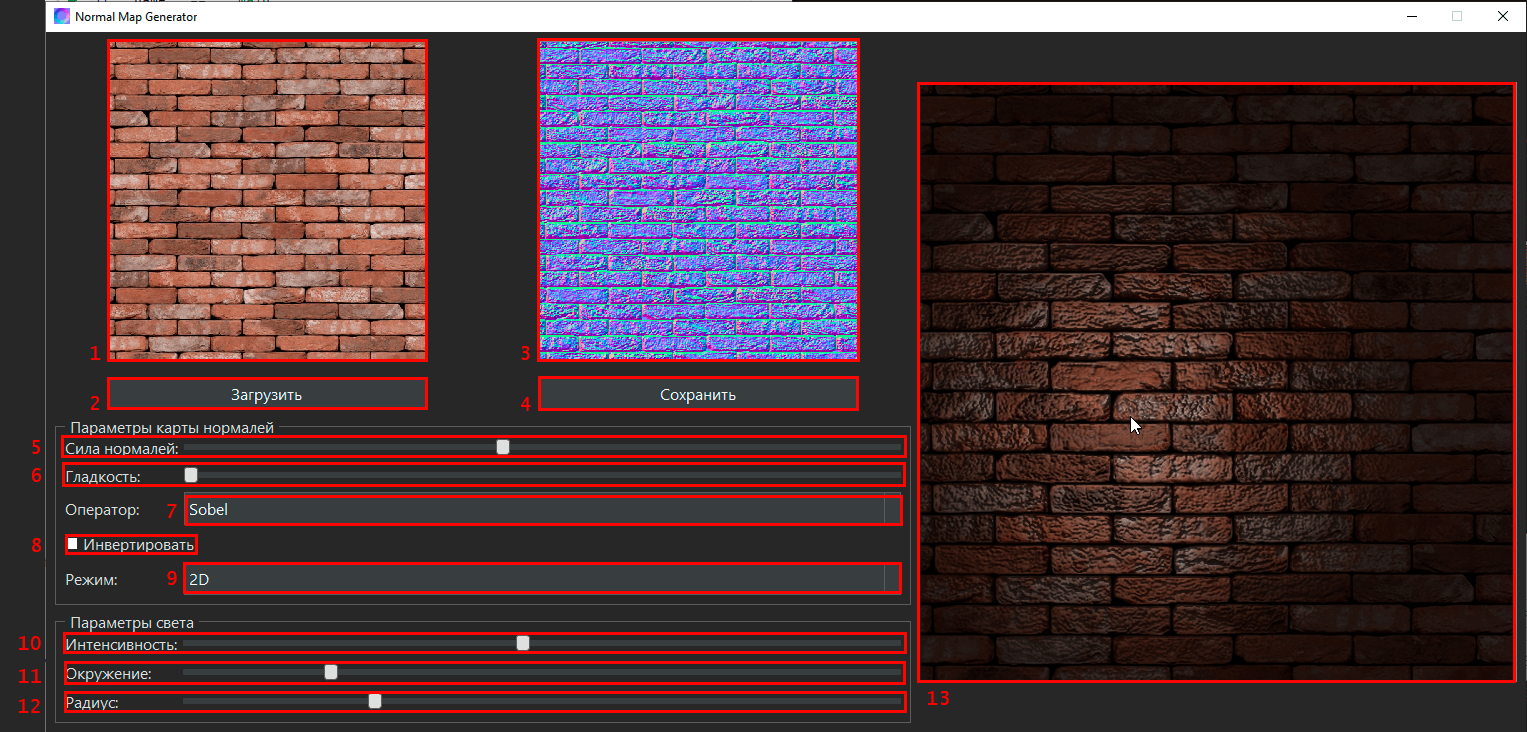
\includegraphics[width=1\linewidth]{interf2}
	\caption{Интерфейс программы}
	\label{interf2:image}
\end{figure}

Элементы интерфейса:
\begin{enumerate}
	\item Окно оригинального изображения. Отображает исходное изображение, загруженное пользователем для генерации карты нормалей.
	\item Кнопка «Загрузить». Открывает диалоговое окно выбора изображения, которое будет использоваться для анализа и генерации нормалей.	
	\item Окно карты нормалей. Показывает сгенерированную карту нормалей на основе оригинального изображения и выбранных параметров.
	\item Кнопка «Сохранить». Сохраняет сгенерированную карту нормалей в выбранное пользователем место.
	\item Ползунок «Сила нормалей». Регулирует интенсивность/амплитуду нормалей. Чем выше значение, тем рельефнее выглядит результат.
	\item Ползунок «Гладкость». Активирует дополнительное влияние глубины на расчет нормалей (если предусмотрена соответствующая логика в коде).
	\item Выпадающий список «Оператор». Позволяет выбрать математический оператор, применяемый для выделения границ (например, Собель, Шарра и др.).
	\item Чекбокс «Инвертировать». При включении инвертирует направление нормалей, меняя визуальное восприятие рельефа.
	\item Выпадающий список «Режим». Позволяет выбрать режим отображения визуализации (2D и 3D).	
	\item Ползунок «Интенсивность». Управляет яркостью источника света при визуализации эффекта освещения.
	\item Ползунок «Окружение». Добавляет равномерное базовое освещение всей сцены для повышения читаемости изображения.
	\item  Ползунок «Радиус». Определяет зону, охватываемую виртуальным «фонариком». Чем больше значение, тем шире область освещённости.
	\item Окно визуализации. Показывает изображение с наложенной картой нормалей, в котором курсор мыши используется как источник света для динамического освещения по карте нормалей.
\end{enumerate}
